\documentclass[crop,tikz,border=10]{standalone}

\usepackage{amsmath, amssymb}
\usetikzlibrary{calc}

\newcommand{\rr}{0.7}
\newcommand{\qq}{0.75}
\begin{document}
    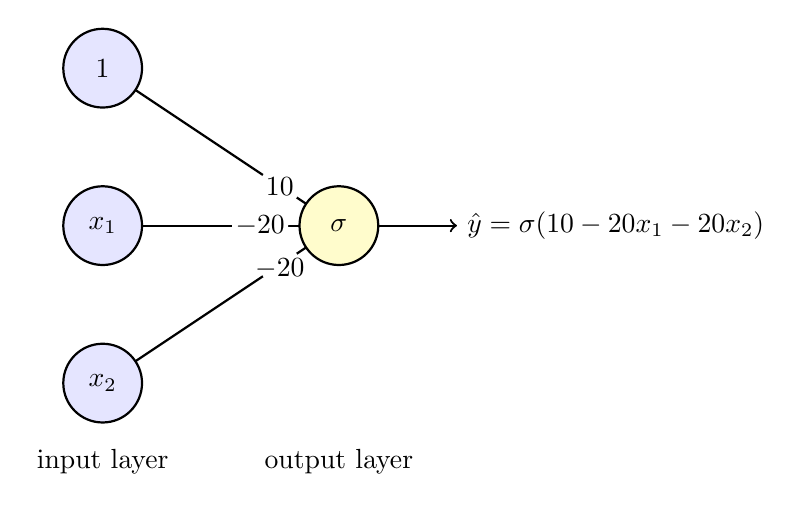
\begin{tikzpicture}

        \draw[thick] (-2, 2) -- (1, 0);
        \draw[thick] (-2, 0) -- (1, 0);
        \draw[thick] (-2, -2) -- (1, 0);
        \draw[thick, ->] (1, 0) -- (2.5, 0) node[right] {$\hat y = \sigma(10 - 20x_1 - 20x_2)$};

        \draw[fill=white, white] ({-2 + \qq*3}, {2 - \qq*2}) circle (0.25);
        \node at ({-2 + \qq*3}, {2 - \qq*2}) {$10$};

        \draw[fill=white, white] ({-2.1 + \rr*3}, 0) circle (0.35);
        \node at ({-2.1 + \rr*3}, 0) {$-20$};

        \draw[fill=white, white] ({-2 + \qq*3}, {-2 + \qq*2}) circle (0.25);
        \node at ({-2 + \qq*3}, {-2.05 + \qq*2}) {$-20$};
        \draw[thick, fill=blue!10] (-2, 2) node {$1$} circle (0.5);
        \draw[thick, fill=blue!10] (-2, 0) node {$x_1$} circle (0.5);
        \draw[thick, fill=blue!10] (-2, -2) node {$x_2$} circle (0.5);

        \draw[thick, fill=yellow!20] (1, 0) circle (0.5);
        \node at (1, 0) {$\sigma$};
        \node at (-2, -3) {input layer};
        \node at (1, -3) {output layer};

        

        % \node[right] at (4.5, 0) {$\hat y =\displaystyle{\begin{cases}0&\text{if $a_1^{[1]}\leq 1/2$}\\[1ex]1&\text{if $a_1^{[1]}> 1/2$}\end{cases}}$};
    \end{tikzpicture}
\end{document}